\documentclass[a4paper]{article}
\usepackage[warn]{mathtext}
\usepackage[utf8]{inputenc}
\usepackage[T2A]{fontenc}

\usepackage[english,russian]{babel}
\usepackage{multicol}
\usepackage{fancyhdr}
\usepackage{graphicx}
\usepackage{microtype}
\usepackage{wrapfig}
\usepackage{amsmath}
\usepackage{floatflt}
\usepackage{geometry} \geometry{verbose,a4paper,tmargin=2cm,bmargin=2cm,lmargin=1.5cm,rmargin=1.5cm}
\usepackage{float}
\usepackage{amssymb}
\usepackage{caption}
\usepackage{epsfig}
\usepackage{newunicodechar}

\begin{document}

\graphicspath{ {pictures/} }

\begin{titlepage}
	\centering
	\vspace{5cm}
    {\scshape\LARGE Московский физико-технический институт\par}
	\vspace{5cm}
	{\scshape\Large Лабораторная работа по фотонике \par}
	\vspace{1cm}
    {\huge\bfseries  Использование твердотельного $YAG:Nd^{3+}$ -лазера с модуляцией добротности для гравировки материалов\par}
	\vspace{1cm}
	\vfill
    \begin{flushright}
        {\large выполнили студенты Б04-852 группы ФЭФМ}\par
        \vspace{0.3cm}
        {\LARGE ...}
    \end{flushright}
	\vfill
Долгопрудный, 2020
% Bottom of the page
\end{titlepage}

\pagestyle{fancy} 
\fancyhead[L]{YAG:$Nd^{3+} \;\;\;$  $\sim  \hat(\, ^{\circ}  \omega  ^{\circ} \, \hat) \sim$}
\fancyhead[R]{Фотоника}
\fancyhead[C]{}
\fancyfoot[C]{ \noindent\rule{\textwidth}{0.4pt} \thepage }


\newpage

\begin{enumerate}
	\item \textbf{Определить величинуэнергии, котораядолжна быть в импульсе ла-зера  на YAG:Nd3+(длина  волны  1.064  мкм)для  того,чтобы испарить 1мм3алюминия} \par
	\item \textbf{Рассчитать расходимость пучка диаметром 1см,генерируемого ла-зером YAG:Nd3+.} \par
	\item \textbf{Оценить минимальный диаметр пучка лазера на YAG:Nd3+при его фокусировке линзой с фокусным расстоянием f= 20 см. В какой области вдоль пучкаразмер перетяжки будет меняться менее чем в $\sqrt{2}$ раз (конфо-кальный параметр), радиус пучка на выходе телескопа лазера 1 см. Счи-тать волновой фронт пучка до линзы плоским.} \par 
	\item \textbf{Рассчитать глубину и размеры отверстия,проделанного в алюми-нии с помощью лазера на YAG:Nd3+, работающего в импульсном режиме. Энергию в импульсе и параметры пучка взять из задач 1 и 3.} \par 
	\item \textbf{Определить время жизни фотона в резонаторе лазера: длина резо-натора –81.5см, длина активного элемента–10см, показатель преломле-ния граната –1.8, одно из зеркал глухое, пропускание другого –20 \%, по-глощение в активном элементе –1 \%.} \par 
	\item \textbf{Определить мощность излучения лазера на $YAG:Nd^{3+}$, работающего в непрерывном режиме. Мощность накачки - 3 кВт, КПД накачки - 20 $\%$, длина резонатора - 81.5 см, длина активного элемента - 10 см, показатель преломления граната 1.8, одно из зеркал глухое, пропускание другого - 20 $\%$, поглощение в активном элементе - 1 $\%$, диаметр активного элемента - 6 мм, время жизни верхнего уровня - 230 мкс, сечение перехода - $2.8 \cdot 10^{-19}\;см^{2}$, энергия между 0 и 3 ураовнями соответсвует энергии фотона с длиной волны 808 нм.} \par 
	\item \textbf{Рассчитать инверсную населенность на момент открытие модулятора для лазера, мощность накачки - 3 кВт, КПД накачки - 20 $\%$, длина резонатора - 81.5 см, длина активного элемента - 10 см, частота импульсов - 50 кГц, диаметр активного элемента - 6 мм, время жизни верхнего уровня - 230 мкс, энергия между 0 и 3 ураовнями соответсвует энергии фотона с длиной волны 808 нм.} \par 
	\item \textbf{Рассчитать длительнсоть импульса лазера, работающего в режиме модуляции добротности с частотой 50 кГц. Мощность накачки - 3 кВт, КПД накачки - 20 $\%$, длина резонатора - 81.5 см, длина активного элемента - 10 см, показатель преломления граната 1.8, одно из зеркал глухое, пропускание другого - 20 $\%$, поглощение в активном элементе - 1 $\%$, диаметр активного элемента - 6 мм, время жизни верхнего уровня - 230 мкс, сечение перехода - $2.8 \cdot 10^{-19}\;см^{2}$, энергия между 0 и 3 ураовнями соответсвует энергии фотона с длиной волны 808 нм.} \par 
	\item \textbf{Как зависит энергия в импульсе лазера от мощности накачки?} \par 

	Для энергии в импульсе известно такое выражение:

	\begin{equation}
		E = \left( \frac{\ln{(R_2)}}{2\ln{((1-L)\sqrt{R_1R_2})}} \right) (N_i - N_f) (V_ah\nu_l),
	\end{equation}
	где $N_f$ - инверсия в момент окончания импульса, она намного меньше $N_i$ - инверсии в момент открытия модулятора, для которого справедливо:

	\begin{equation}
		N_i = \frac{P_{нак} \eta}{Slh\nu} \tau \left ( 1 - e^{-t/\tau} \right)
	\end{equation}

	Видим, что $N_i \sim P_{нак}$, следовательно  $E \sim P_{нак}$, зависимость линейная, построим ее график (рис. \ref{E_p(P)}):

	\begin{figure}[H]
		\begin{center}
			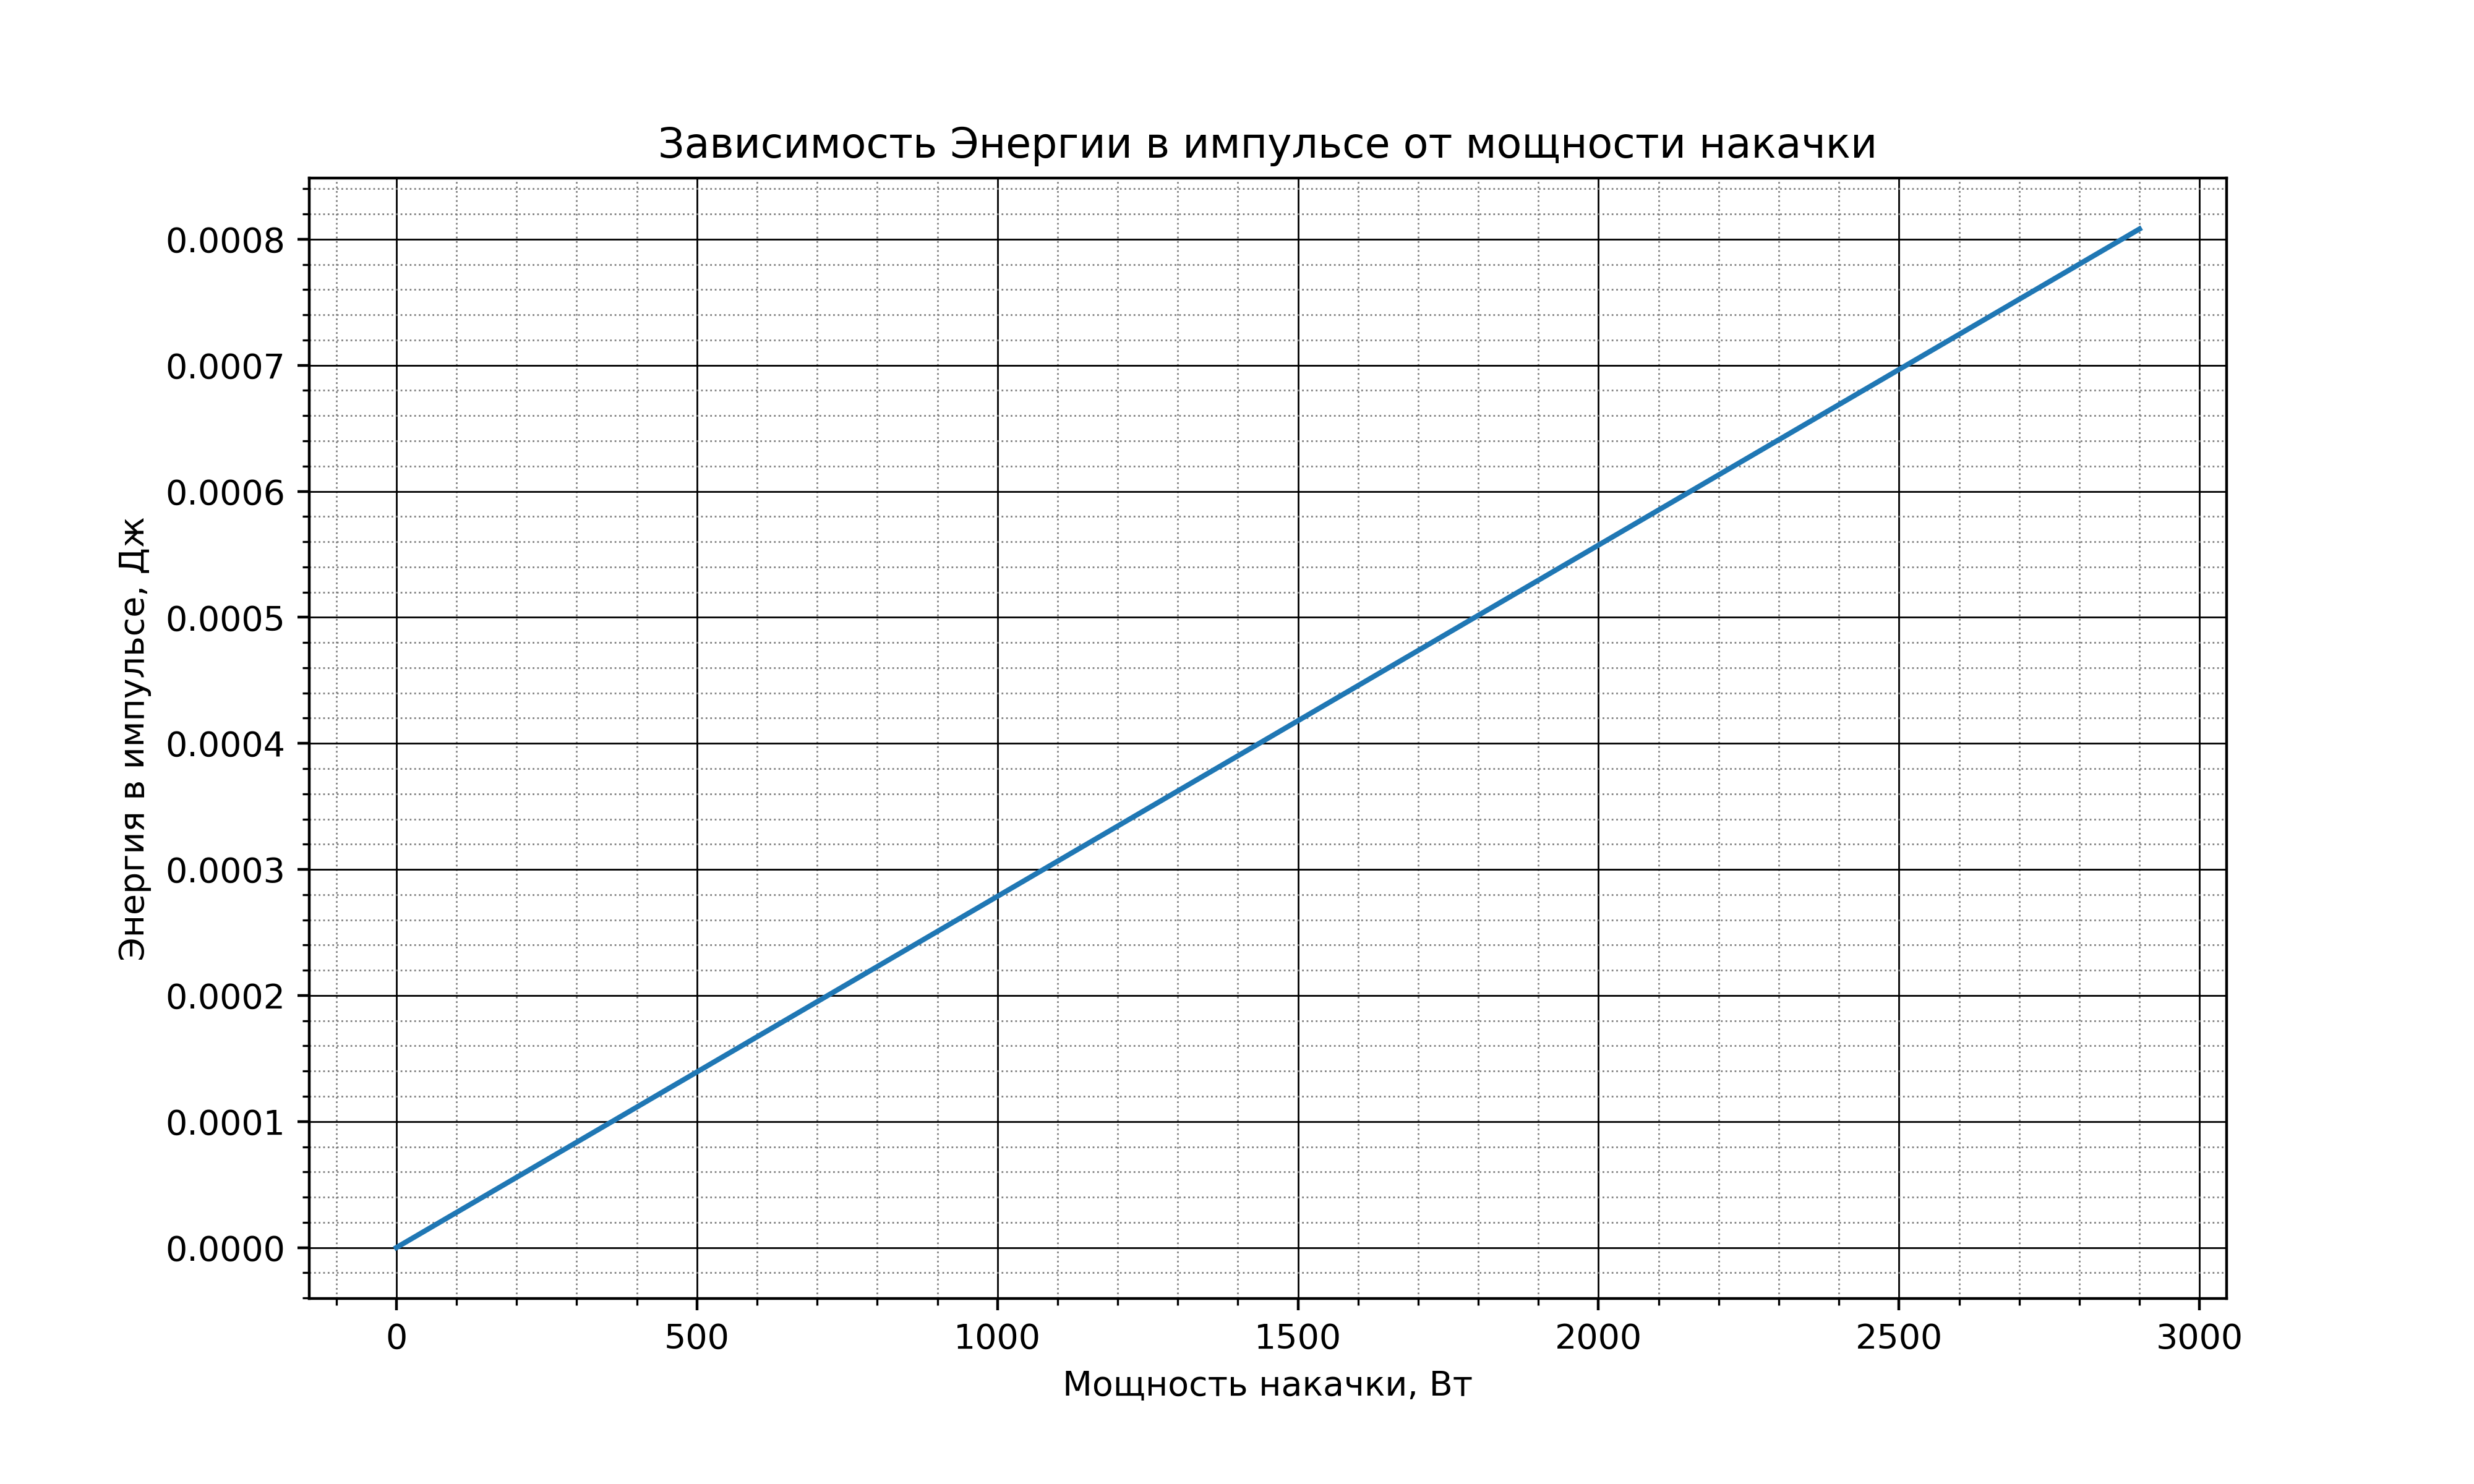
\includegraphics[scale = 0.5]{E_p(P).png}
			\caption{}
			\label{E_p(P)}
		\end{center}
	\end{figure}

	\item \textbf{Показать зависимость энергии излучения в импульсе в зависимости от частоты открывания модулятора.} \par 

	Для энергии в импульсе имеем:

	\begin{equation}
		E = \left( \frac{\ln{(R_2)}}{2\ln{((1-L)\sqrt{R_1R_2})}} \right) (N_i - N_f) (V_ah\nu_l),
		\label{energy}
	\end{equation}

	где $N_i$ определяется:

	\begin{equation}
		N_i = \frac{P_{нак} \eta}{Slh\nu} \tau \left ( 1 - e^{-1/\nu \cdot \tau} \right)
	\end{equation}

	Получяем: 

	\begin{equation}
		N_i \sim 1 - e^{-1/ \nu}
	\end{equation}

	Что является убывающей функцией от частоты открывания модулятора. Этот вывод можно сделать их сообьражений, что чем чаще открывается модулятор, тем меньше будет инверсия 
	заселенности, тк будет меньше времени для накачки, соответсвенно чем меньше заселенность, тем меньше фотонов мы получим и энергия излучения будет меньше. Построим график на рис. \ref{E_p(nu)}

	\begin{figure}[H]
		\begin{center}
			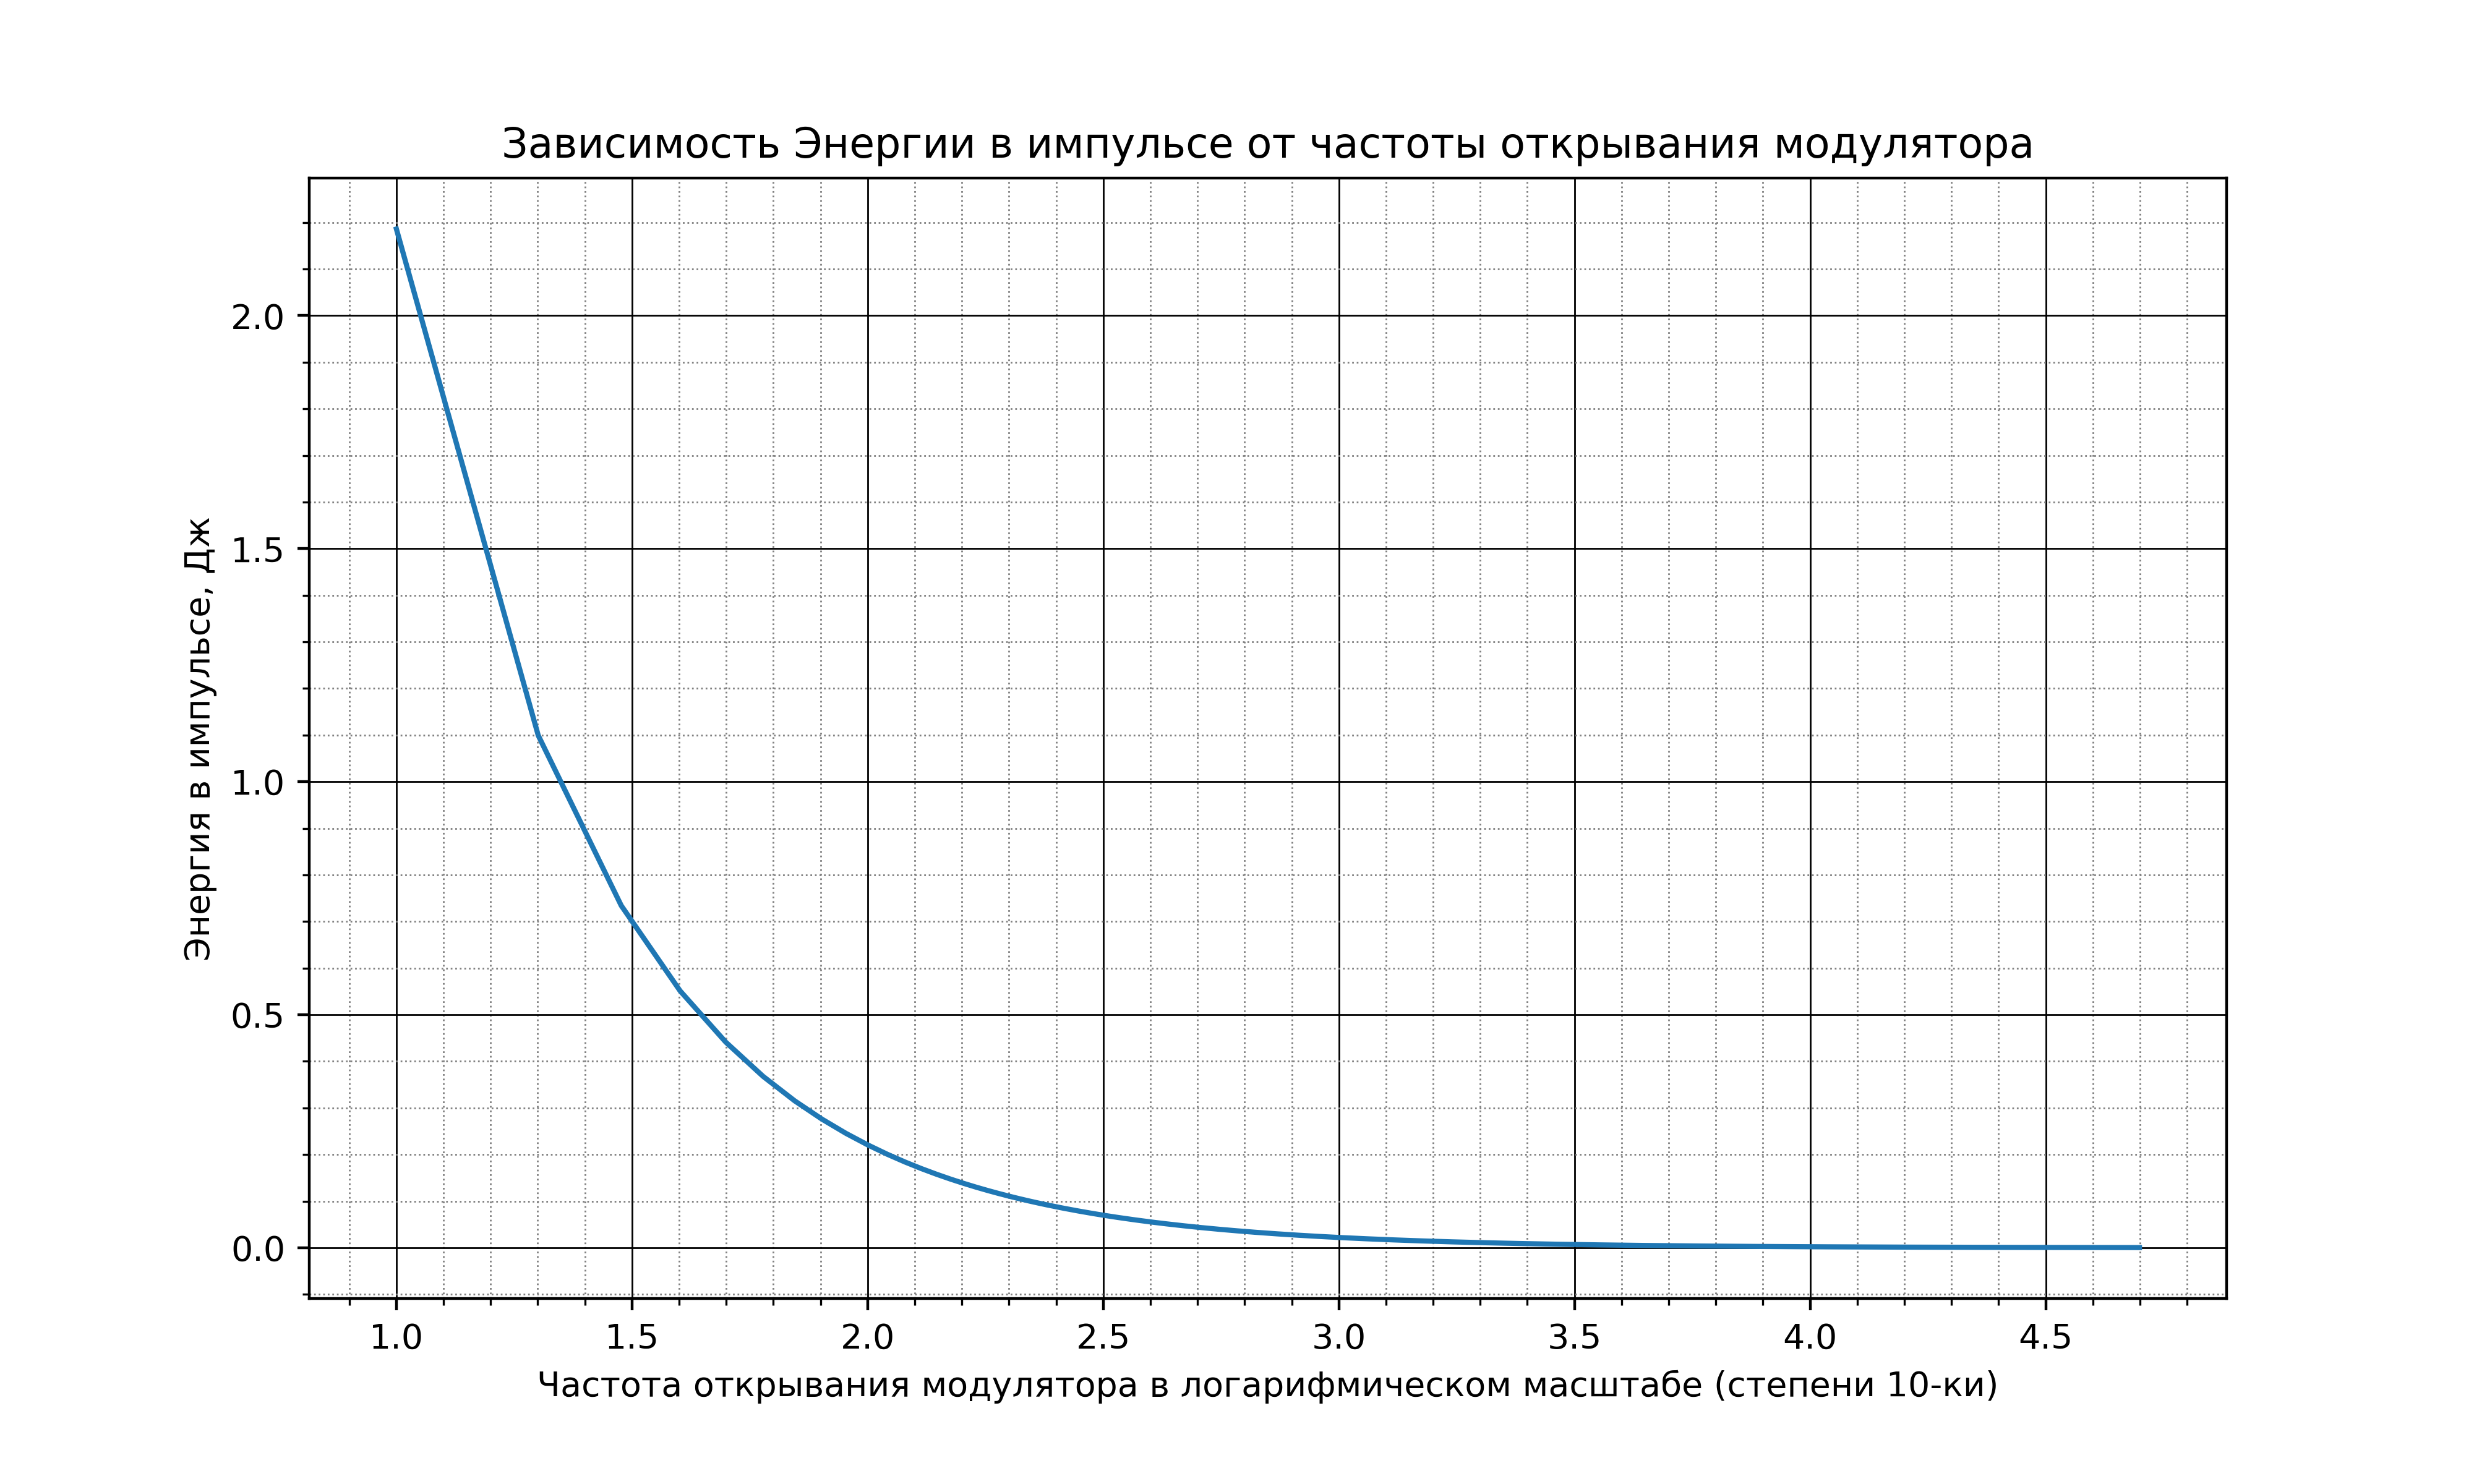
\includegraphics[scale = 0.5]{E_p(nu).png}
			\caption{}
			\label{E_p(nu)}
		\end{center}
	\end{figure}

	\item \textbf{Рассчитать энергию в импульсе и пиковую мощность для лазера из задачи 7.} \par

	По формуле (\ref{energy}) определим энергию в импульсе:

	$$E_p = 0.00737\; Дж$$

	
	Значение мощности излучения в импульсе:

	\begin{equation}
		P_p = \left ( \frac{-\ln{(R_2)} c}{2 L_e} \right) (h \nu_l) \varPhi_p
	\end{equation}
	
	Пик импульса достижим при максимуме числа фотонов, который достигается при $N_p = N_0$, что видно из графиков рис. \ref{modulation}

	\begin{figure}[H]
		\begin{center}
			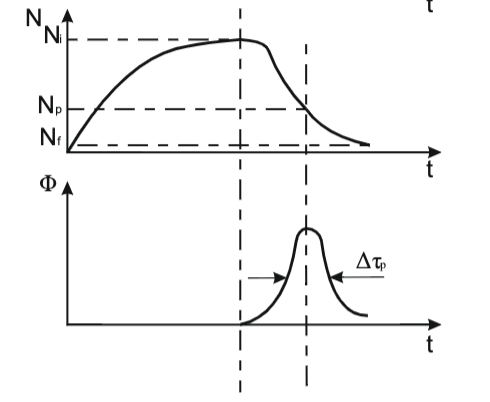
\includegraphics[scale = 0.7]{modulation.png}
			\caption{Зависимость от времени ивнерсии населенностей и числа фотонов}
			\label{modulation}
		\end{center}
	\end{figure}

	\begin{equation}
		\varPhi_p = V_a N_p \left ( \frac{N_i}{N_p} - \ln{\frac{N_i}{N_p}} - 1 \right)
	\end{equation}

	Тогда получим для пика мощности импульса:

	$$P_p = 42.42 кВт$$

\end{enumerate}


\end{document}